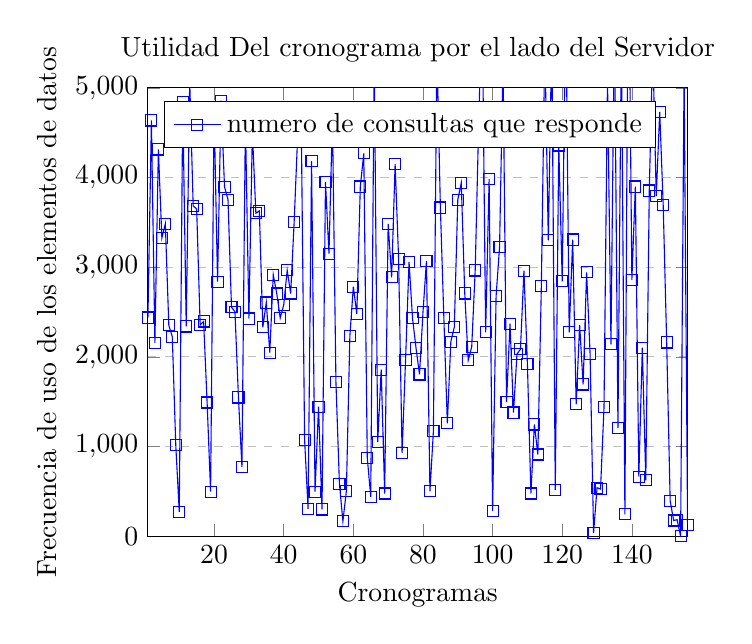
\begin{tikzpicture}
\begin{axis}[
    title={Utilidad Del cronograma por el lado del Servidor},
    xlabel={Cronogramas},
    ylabel={Frecuencia de uso de los elementos de datos},
    xmin=1, xmax=156,
    ymin=0, ymax=5000,
    xtick={},
    ytick={},
    legend pos=north west,
    ymajorgrids=true,
    grid style=dashed,
]

\addplot[
    color=blue,
    mark=square,
    ]
    coordinates {
%UTILIDAD TOTAL
%(cronograma, numero cues que usan al cronograma)
(1,2438)
(2,4637)
(3,2155)
(4,4313)
(5,3326)
(6,3483)
(7,2351)
(8,2225)
(9,1013)
(10,272)
(11,4840)
(12,2339)
(13,5075)
(14,3683)
(15,3650)
(16,2356)
(17,2395)
(18,1491)
(19,497)
(20,4761)
(21,2838)
(22,4858)
(23,3896)
(24,3754)
(25,2554)
(26,2503)
(27,1547)
(28,772)
(29,4646)
(30,2427)
(31,4509)
(32,3602)
(33,3628)
(34,2330)
(35,2606)
(36,2047)
(37,2916)
(38,2706)
(39,2434)
(40,2579)
(41,2965)
(42,2707)
(43,3505)
(44,4459)
(45,4769)
(46,1077)
(47,301)
(48,4184)
(49,496)
(50,1444)
(51,298)
(52,3952)
(53,3151)
(54,4675)
(55,1719)
(56,584)
(57,167)
(58,503)
(59,2231)
(60,2783)
(61,2481)
(62,3899)
(63,4270)
(64,875)
(65,440)
(66,5392)
(67,1049)
(68,1858)
(69,476)
(70,3484)
(71,2887)
(72,4149)
(73,3093)
(74,927)
(75,1968)
(76,3059)
(77,2429)
(78,2100)
(79,1804)
(80,2496)
(81,3071)
(82,500)
(83,1173)
(84,5437)
(85,3665)
(86,2433)
(87,1259)
(88,2168)
(89,2332)
(90,3752)
(91,3940)
(92,2707)
(93,1962)
(94,2112)
(95,2964)
(96,4605)
(97,5992)
(98,2273)
(99,3982)
(100,281)
(101,2677)
(102,3226)
(103,5309)
(104,1496)
(105,2370)
(106,1379)
(107,2032)
(108,2085)
(109,2962)
(110,1916)
(111,476)
(112,1246)
(113,911)
(114,2789)
(115,5500)
(116,3300)
(117,5605)
(118,513)
(119,4358)
(120,2842)
(121,6088)
(122,2273)
(123,3308)
(124,1470)
(125,2356)
(126,1692)
(127,2942)
(128,2035)
(129,37)
(130,541)
(131,525)
(132,1439)
(133,5095)
(134,2140)
(135,5838)
(136,1207)
(137,5663)
(138,244)
(139,6921)
(140,2860)
(141,3899)
(142,664)
(143,2102)
(144,622)
(145,3855)
(146,5466)
(147,3792)
(148,4733)
(149,3690)
(150,2161)
(151,394)
(152,175)
(153,184)
(154,0)
(155,5170)
(156,129)
(157,4789)
    };
    \legend{numero de consultas que responde}

\end{axis}
\end{tikzpicture}

